\chapter{Contexte}
\label{chap:contexte}

Les liquides ioniques sont des éléments beaucoup utilisés en chimie. Ils permettent notamment de stocker de l'énergie mais disposent aussi de nombreuses autres applications.

Les liaisons ioniques s'obtiennent par l'attraction de deux ions de charge opposée. Les ions de charges positives et négatives sont respectivement appelés : cation et anion. Généralement, les cations sont métalliques tandis que les anions ne le sont pas. Un ion est composé d'un ou plusieurs atomes chargés électriquement.

Les possibilités de liaisons sont probablement infinies et leurs propriétés diffèrent pour chaque composition. Dans notre cas, la particularité qui nous intéresse est le point d'ébullition. Si on voulait obtenir cette information par expérience, il faudrait compter en jour le temps et les ressources consommées seraient importantes. L'objectif de ce travail de semestre est d'estimer la température d'ébullition d'un liquide ionique afin de concentrer le temps et les ressources de l'institut ChemTech de la HEIA-FR sur des liaisons validées par l'outil au préalable.

Ce travail sera utilisé comme outil de base pour un projet visant à stocker ou récupérer de l'énergie dans les phases de changements d'états d'un liquide ionique. Le but est d'y insérer en entrée le \acrfull{smiles} de l'anion et du cation et on obtiendra la température estimée.

L'écriture \acrshort{smiles} est utilisée en chimie pour décrire des molécules. Cette écriture permet de reconstruire le modèle 3D ou 2D comme ci-dessous :
\begin{center}
   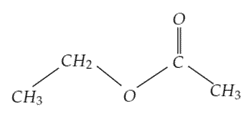
\includegraphics[height=20mm]{img/smiles_example.png}
   \captionof{figure}{Exemple de \acrshort{smiles}}
\end{center}

 
Il existe une librairie python qui permet de récupérer les informations issues d'un \acrshort{smiles}.

Ce projet a déjà été amorcé par Mme Yerly et un étudiant réalisant master de mathématiques à la HEIA-FR. Ils ont réussi à reproduire les résultats obtenus dans une étude à l'aide de la base de données fournie par cette dernière et vérifier par la base de données de l'école. Ce modèle était basé sur l'algorithme SVM (Support Vector Machine).

Ces algorithmes ont besoin de données d'entrées et de cibles. Son but sera de faire le lien entre les différents paramètres insérés et la cible la plus probable.

Dans un second temps, on pourrait aussi imaginer améliorer l'outil en rajoutant une surcouche qui déterminera le meilleur liquide ionique pour un objectif donné ou la possibilité de prédire d'autres propriétés.
